\documentclass[11pt,letterpaper]{article}
\usepackage{acl2013}
\usepackage{times}
\usepackage{latexsym}
\usepackage{amsmath}
\usepackage{amssymb}
\usepackage{amsthm}
\usepackage{enumitem}
\usepackage{verbatim}
\usepackage{mathtools}

\usepackage{graphicx}
\usepackage{algorithm}
\usepackage{algorithmic}

\DeclareMathOperator*{\argmax}{arg\,max}

%\usepackage{authordate1-4}
\usepackage{multirow}

\usepackage{color,soul}
\usepackage[usenames,dvipsnames,svgnames,table]{xcolor}
\newcommand{\Note}[1]{}
\renewcommand{\Note}[1]{\hl{[#1]}}
\newcommand{\NoteSigned}[3]{{\sethlcolor{#2}\Note{#1: #3}}}
\newcommand{\RemoveFF}[1]{\NoteSigned{Remove (FF)}{Crimson}{#1}}
\newcommand{\NoteFF}[1]{\NoteSigned{FF}{LightBlue}{#1}}
\newcommand{\NoteJE}[1]{\NoteSigned{JE}{LightGreen}{#1}}

\setlength\titlebox{6.5cm}    % Expanding the titlebox


\title{A Virtual Manipulative for Learning Log-Linear Models}


\author{
	 Author 1\\
	    XYZ Company\\
	    111 Anywhere Street\\
	    Mytown, NY 10000, USA\\
	    {\tt author1@xyz.org}
	  \And
	  Author 2\\
	    XYZ Company\\
	    111 Anywhere Street\\
	    Mytown, NY 10000, USA\\
	    {\tt author1@xyz.org}
 }
  
\date{}

\begin{document}

\maketitle

\begin{abstract}
We present a virtual manipulative for regularized conditional log-linear models. 
\end{abstract}

\section{Introduction}\label{sec:intro}
except for reading of data files, purely client-side $\Rightarrow$ very easy to set-up;
open-source;
data input format makes it extensible;
individual lessons can be tailored (e.g., hide/show buttons, different tool-tips for lessons)

Why do we focus on shapes, rather than words? \NoteFF{maybe we can argue via virtual manipulatives}

\NoteFF{what is the history of virtual manipulatives in teaching CS? NLP?} the HMM spreadsheet \cite{eisner-2002-tnlp}

\section{Regularized Conditional Log-Linear Models}
Our aim is to provide an intuitive understanding of regularized conditional log-linear models. Given $K$ features $f_k$ representing $N$ data points $\{( x_i, y_i)\}_{i=1}^N$, we are interested in estimating distributions 
\begin{equation}
\hat{p}_{\vec{\theta}}\left(y\ \mid\ x\right) = \frac{u(x, y)}{\sum_{y'} u(x,y')},
\label{eqn:conditional_loglin}
\end{equation}
where $u(x,y)$ represents the unnormalized probability
\begin{eqnarray}
u(x,y) & = & \exp{\left(\vec{\theta}\cdot \vec{f}(x,y)\right)}\\
& = & \exp{\left(\sum_{k=1}^K \theta_k f_k(x,y)\right)}.
\end{eqnarray}
As our model $\hat{p}_{\vec{\theta}}$ is fully described by the feature weights $\vec{\theta}$, we find the weights that maximize the regularized conditional log-likelihood \eqref{eqn:reg_ll}:
\begin{equation}
F\left(\vec{\theta}\right) = \sum_{i=1}^N \log{\hat{p}_{\vec{\theta}}\left(y_i\ \mid\ x_i\right)} - C \cdot R\left(\vec{\theta}\right).
\label{eqn:reg_ll}
\end{equation}
Here, $C \ge 0$ is the regularization penalty for the regularizer $R(\vec{\theta})$. We will generally refer to the \textbf{full model} as that of \eqref{eqn:conditional_loglin} with objective \eqref{eqn:reg_ll}.

However, because the full model may present too many subtleties to be grasped all at once, we also consider ``simplified'' global models $\hat{p}_{\vec{theta}}\left(y\right)$. These context-nescient models allow students to focus initially on understanding some of the core underlying concepts of exponential models, such as feature interations and weight tradeoffs, before progressing to conditioned models.

\NoteFF{move to a later section} Using $\tilde{p}$ to represent the empirical distribution, the gradient of \eqref{eqn:reg_ll} is, in general,
\begin{equation}
\nabla_{\vec{\theta}} F = 
\mathbb{E}_{\tilde{p}}\left[\vec{f}(x,y)\right] 
- \mathbb{E}_{\hat{p}}\left[\vec{f}(x,y)\right]
- C \nabla_{\vec{\theta}}R(\vec{\theta}).
\end{equation}
We consider models where $R(\vec{\theta}) = \vec{0}$ (no regularization), $R(\vec{\theta}) = \|\vec\theta\|_1$, and $R(\vec{\theta}) = \|\vec{\theta}\|_2^2$: we special-case the optimizer to handle the non-differentiable $\ell_1$ regularization, thus providing a friendly educational environment in which the student may explore the differences between $\ell_1$ and $\ell_2$ regularization.

\section{Our Notes}
\NoteFF{These are simply copied from the Google doc titled ``600.465: Maxent Notes.'' This section could be retitled general pedagogical aims, or something of the sort.}
\begin{itemize}
\item If the “striped” feature is predicted to occur less often than it actually does, you should raise its weight.
\item It’s possible to overfit the training data.  Regularization compensates for that and can in fact make you underfit.
\begin{itemize}
\item In particular, weights may zoom off to +infinity or -infinity if a feature is always or never present on the *observed* examples (may need to cook special datasets for this)
\end{itemize}
\item Interactions:
\begin{itemize} 
\item Raising one weight may reduce or reverse the need to raise other weights.  This can be seen by watching the gradient as we slide the slider.
\item Can share features across conditions and this helps regularizer even if likelihood is the same
\item Features that only fire on conditions have no effect on conditional distribution
\item Feature conjunctions: fewer vs. more features
\item Feature that everything/nothing has --- weights go to $\pm \infty$
\item Opposing features, e.g., solid vs striped, where there are only 2 options (or, red vs. blue)
\end{itemize}
\item Likelihood always goes up if you follow gradient
\begin{itemize}
\item gradient = observed - expected count (- regularizer)
\item This is evident in the LL-bar at the top
\end{itemize}
\item LL is maximized when you match the empirical (except for overfitting?)
\item Frequent conditions more influential
\item Some distributions can't be matched --- but you get generalization
\item The initial setting where all weights = 0 gives the uniform distribution.
\begin{itemize}
\item Some further understanding of the entropy view?  (See below.)
\end{itemize}
\end{itemize}

\NoteFF{Make sure to address this:} We should note that we are \textit{not} concerned with computational issues here, e.g., that of tractably computing the per-context normalization factor. While efficiently computing the normalization factor is a crucial component to practical log-linear models, our primary concern is to provide an intuitive understand. \NoteFF{work on the wording here...}

\NoteFF{It's also important to talk about convexity of the objective.} That is, we'll always find a unique $\vec{\theta^*}$ that solves \eqref{eqn:reg_ll}.

\section{Virtual Manipulative Overview}
See Figure \ref{fig:lesson1} for a screenshot.
\begin{figure*}[t]
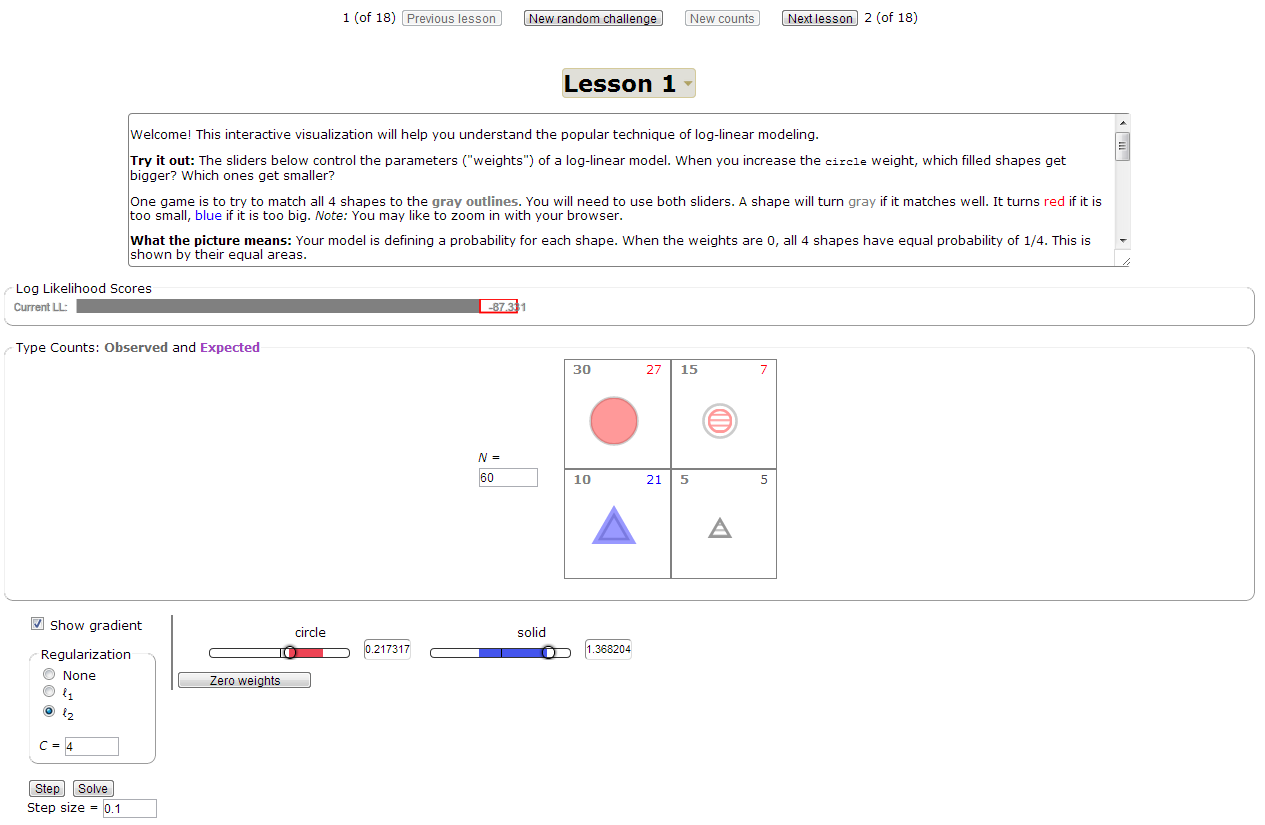
\includegraphics[scale=.5]{images/lesson1-grad-moved-nonewcounts-ell2-c4.PNG}
\caption{Screenshot of the first lesson from the virtual manipulative.}
\label{fig:lesson1}
\end{figure*}

\section{Usability}
\begin{description}
\item[``New Counts'' button] The other use is to help the user experiment with datasets of different sizes, by changing N to scale the counts and then clicking "New counts."
\end{description}

\subsection{Data description}
\begin{description}
\item[Required]

\begin{itemize}
\item a set of contexts (if missing, will be assumed to contain only one context)
\item a set of features; some of these may be marked as hidden
\item for each context, a set of events and visual positions for them \NoteFF{explain why this visual positioning is pedagogically important, i.e., aligning \texttt{circles} vs. \texttt{triangles}, and \texttt{solid} vs. \texttt{striped} can make feature contrasts stand out more}
\end{itemize}

\item[Optional]

\begin{itemize}
\item weights for some or all features (if missing, will be imputed from the prior N(0,I) and the supplied count vectors)
If no counts are supplied, then imputation is equivalent to simple sampling from N(0,I).
More generally, imputation requires MH sampling of the feature weights (and it’s wise to initialize the sampler to a MAP estimate found by the solver).  We may not implement this case immediately, in which case the weights may stay unknown.  In that case we have to gray out a couple of buttons and treat contexts without count vectors as if they had no observations.
\end{itemize}

\item[Not done] \NoteFF{sadly, these didn't get tended to}
\begin{itemize}
\item visual positions for all visible and hidden features (if missing, will be filled in heuristically)

for each context, a total count $N_x$ (if missing, will be imputed from an integerized gamma prior and the supplied event counts and the weights)
In practice, we can forbid the lesson-maker from supplying only some of the event counts in a given context.  In that case, either the whole count vector is given and $N_x$ is just the sum, or none of the count vector is given and $N_x$ is sampled from the gamma.
for each (context, event) pair, a count (any missing counts for this context will be imputed)
In practice, we can forbid the lesson-maker from supplying only some of the event counts in a given context.  In that case, if any of this count vector is missing, then the whole thing is missing, and we can impute it simply by sampling $N_x$ events from the distribution defined by the model weights.
\end{itemize}
\end{description}


\bibliography{tnlp}
\bibliographystyle{acl}

\end{document}
